Lämpöpumppujen käyttö kiinteistöjen lämmitykseen kasvattaa suosiotaan(Lähde, lukumäärät). Lämpöpumppu saattaa olla kiinteistön ainut lämmitysmuoto, tai se saattaa toimia toisten lämmitysjärjestelmien rinnalla. Lämpöpumpuilla voidaan korvata vanha järjestelmä, millä on vaikutusta kiinteistön lämmityksen aiheuttamaan sähkönkulutuksen luonteeseen.

\section{Lämpöpumpun toimintaperiaate}
  Lämpöpumpun eli jäähdytyskoneen toimintaperiaate on käänteinen lämpövoimakoneelle. Lämpöpumppu siirtää lämpöenergiaa viileämmästä ympäristöstä lämpimämpään.

  Lämpöpumpun perusrakenne koostuu kompressorista, lauhduttimesta, paisuntaventtiilistä ja höyrystimestä, joiden välillä kiertää kylmäaine. Järjestelmä on kuvattu kuvassa \ref{fig:hptp}. Matalassa paineessa oleva kylmäaine höyrystyy viileämmässä tilassa sijaitsevassa höyrystimessä ja vastaannottaa lämpöenergiaa. Höyrystynyt kylmäaine johdetaan lauhduttimeen ja sen paine nostetaan kompressorin avulla korkeammaksi, jolloin sen lämpötila nousee. Korkeassa paineessa ja lämpötilassa oleva kylmäaine luovuttaa lämpöenergiaa lauhduttimen välityksellä lämpimään ympäristöön, jolloin osa siitä nesteytyy. Nesteytynyt kylmäaine virtaa paisuntaventtiilin kautta takaisin höyrystimeen. Paisuntaventtiilissä kylmäaineen paine ja täten myös lämpötila laskevat.

  \begin{figure}
    \centering
    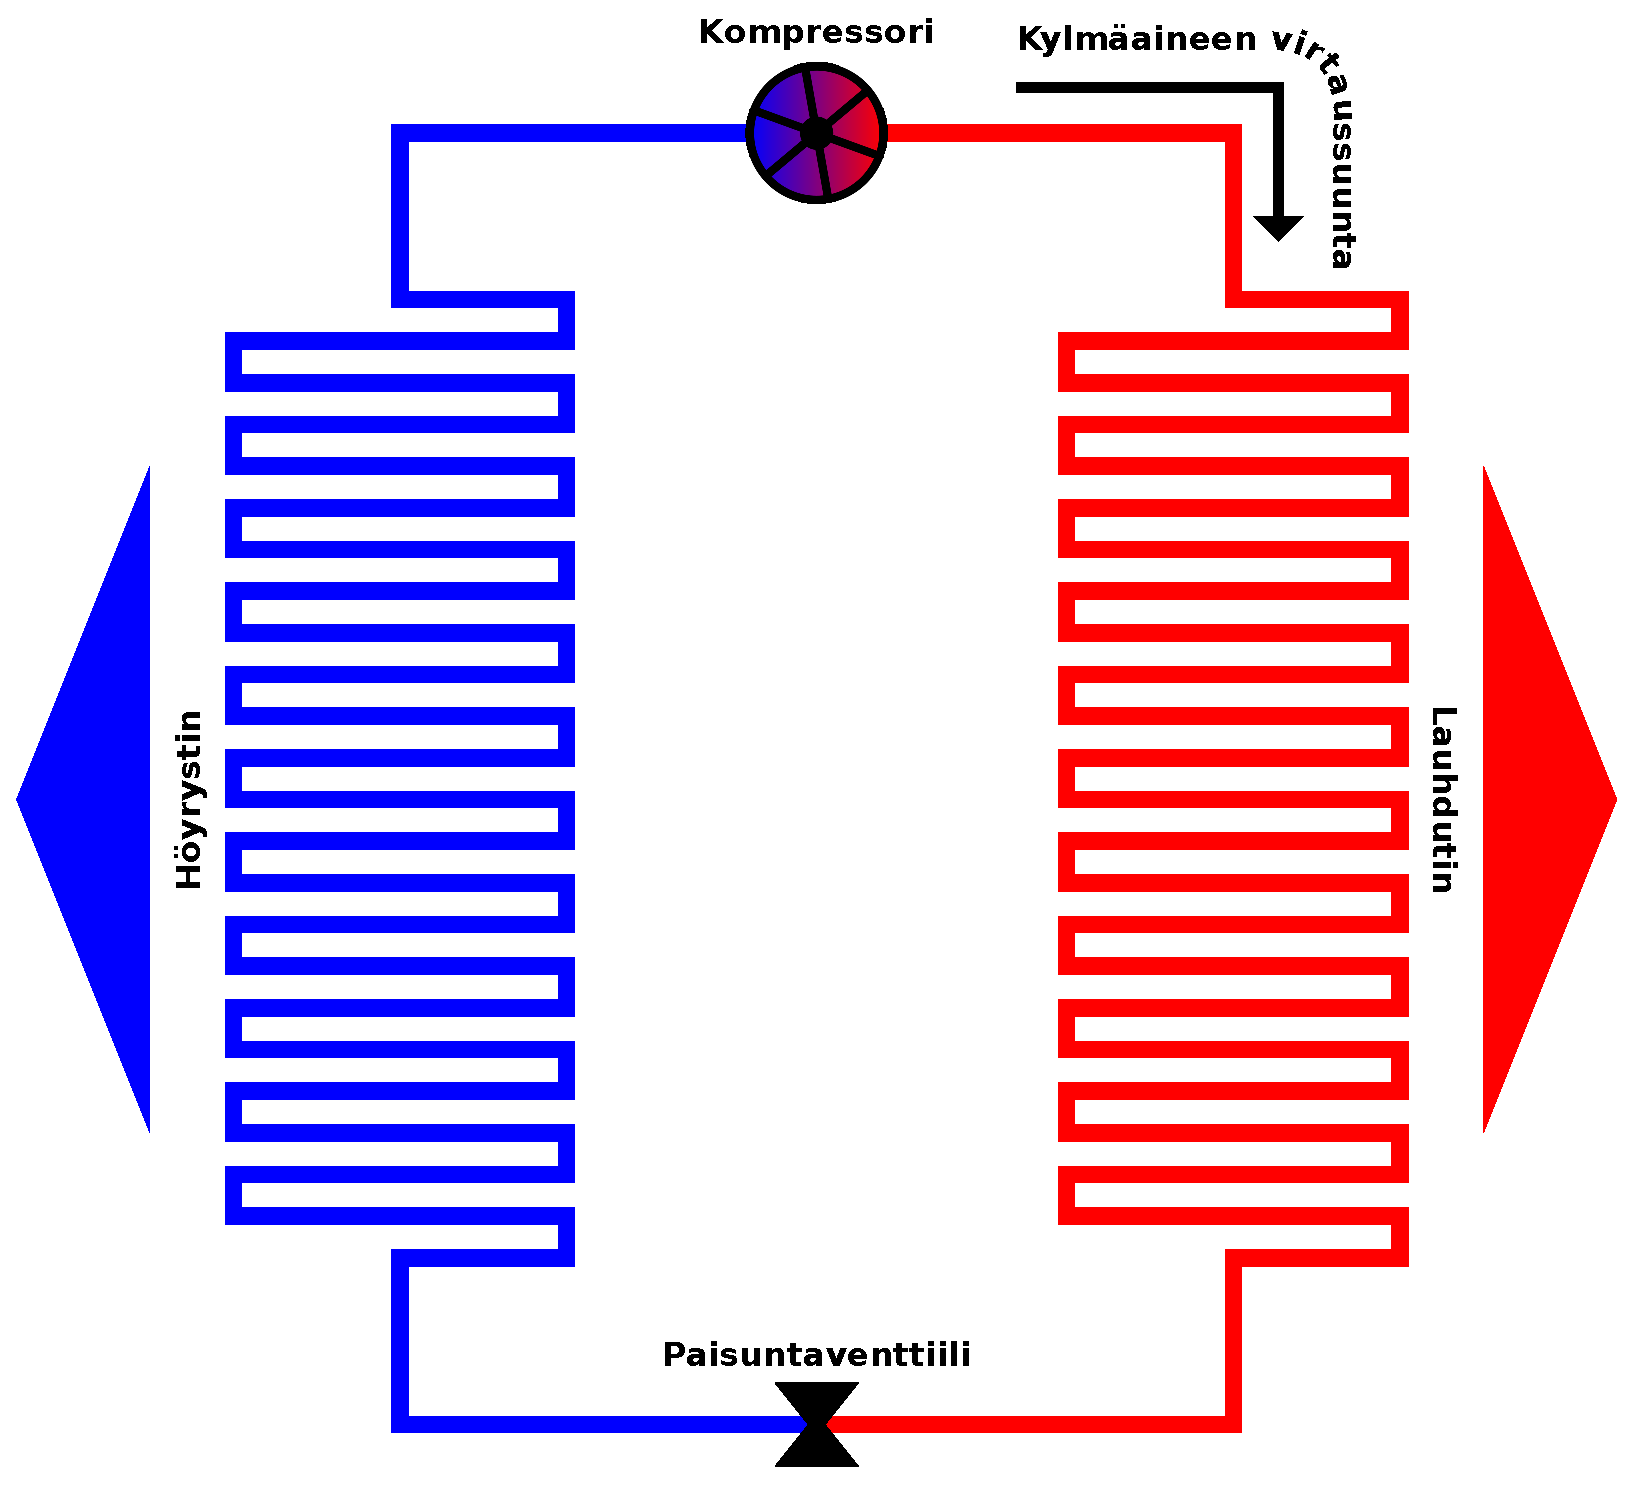
\includegraphics[width=0.5\textwidth]{figures/hp}
    \caption{Lämpöpumpun toimintaperiaate}
    \label{fig:hptp}
  \end{figure}
